\section{Methodology}
\label{sec:met}

Being the already cited problem the creation of a P2P (Peer to Peer) application, it is vital to first identify the aspects that a P2P program normally fulfills, in order to work correctly. A P2P program, essentially, is an application that is used to share content through the network. Its most important difference from other downloading methods (FTP servers etc.) is that there is no central node in which content is downloaded from and uploaded to. The content flows through a decentralized network of nodes, clients, who simultaneously work as servers (or seeders, because they seed content) and downloaders (leechers). They are also servers in the P2P network, but they have a different role:
 
\begin{description}
 \item [Servers] Servers are used to identify and contact different clients between them. They do not take part in the actual process of downloading or uploading content, that is the clients' job. If the server infrastructure falls down, it can be replaced with a new one; no data is lost.
 \item [Clients] The core relies on the clients. Those are the responsible for downloading and uploading content, all the heavy traffic is done between clients, the server only helps meeting clients with similar interests. Normally, clients can stop and resume processes, and hold different processes at the same time (both uploads and downloads). More advanced features consists of bandwidth usage and a virtual crediting system to give priority to clients who share most. 
\end{description}

Thus, if we leave the more advanced features aside, we have already defined what our program should do, with its two main parts: servers and clients. The server (a main one is enough to build a prototype) is the responsible to put clients together and clients are responsible for moving content. The client is the one an average user would use, so it is the one we will focus on. The server needs no user interaction.

%Casos de uso diagrama
\begin{figure}
   \centering
   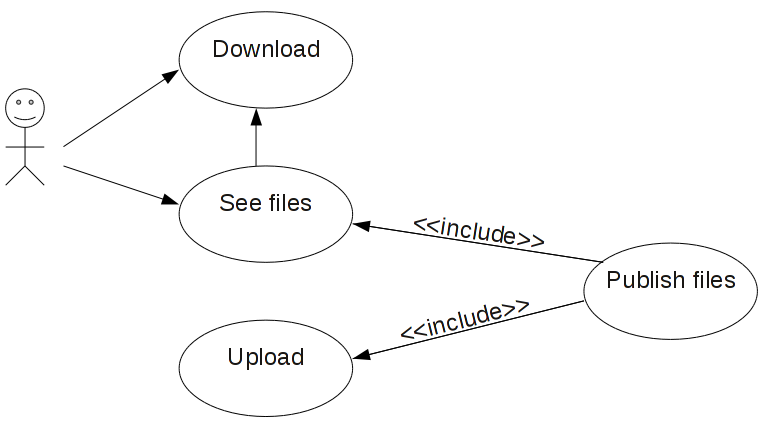
\includegraphics[scale=0.5]{irudiak/usercase.png}
   % Laster-markak gehitzeko menua
   \caption{User Case diagram of the P2P client}
   \label{fig:usercase}
\end{figure}

The diagram no. \ref{fig:usercase} shows the User Case diagram of the client, from the point of view of the user. When the user starts the program, receives from the server the list of the files available (the ones that other users have published) and chooses which one of the files wants to download. Without the user's consent, the files he or she is sharing are sent to other clients and if other clients want one of the files the user has, the upload of the content will also start automatically. Different uploading and downloading processes can be carried at the same time. 

It has to be mentioned though, that the user can control the content he or she wants to upload, but not through this application. All the content the user wishes to share is stored in a directory called \texttt{ongoing}, so the user can use the Operating System to put or remove different files in the directory, but as said, it cannot be done using the program. Likewise, all the downloaded content is stored in a directory called \texttt{incoming} and once the file is downloaded, it is the user who places the file in the directory he or she wishes to.

Before continuing with in-depth analysis and design of the application, it has to be cleared how many connections are there going to be. It has been noted before, that the main connections (the ones sharing content goes through) are between clients and that clients only turn to servers to know what files are being shared. Once the desired file has been selected and download starts from another client (or various, depending on the case) the server just keeps updating the downloadable file list, based on the clients that connect and disconnect. 

\begin{figure}
   \centering
   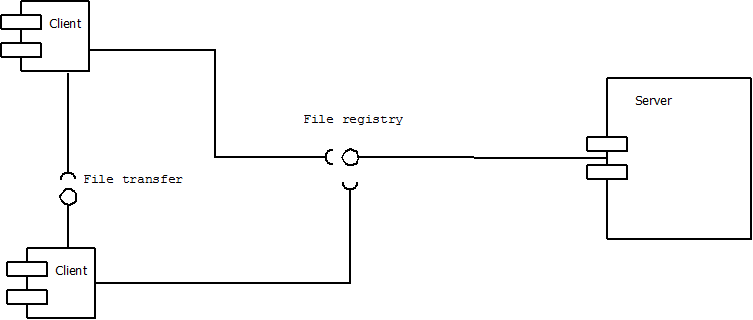
\includegraphics[scale=0.5]{irudiak/Loturak.png}
   % Laster-markak gehitzeko menua
   \caption{Connections in the P2P system}
   \label{fig:lotura}
\end{figure}

What has been told previously is summarized by the figure no. \ref{fig:lotura}. The diagram shows how the clients connect to the server to register files (and to receive the last version of the list showing the available files), and once they have selected what file to download, the server puts in contact the two clients (here the simplest case is shown, but more clients can be involved in the process), the seeder (the one who uploads) and the leecher (the one who downloads) start transferring content, but they still maintain contact with the server, to update the file list and to have the possibility to connect to other clients.

Finally, it is important to note that although general diagrams of the working programs have been done \textit{before} the application was developed, technically deeper diagrams that come later have been outlined \textit{after} the application was developed, in order to be as accurate as possible. For the sake of cleanness, and to ease things as much as possible to the reader, diagrams that were outlined in order to guide the development of the program have not been included in this report, as those diagrams have gone through numerous changes from the original version until the final one.

Thus, programming started early enough to make non-structural changes to the main design, but the main aspects of the program remained the same. The IDL file, for instance, was defined early in the analysis stage and luckily, there has been no need to change it all along the development phase:

\begin{lstlisting}[language=IDL]
module erabilgarriak{
	struct FileData{
		string name;
		long long size;
		string hash;
	};
	interface DownloadFile{
		typedef sequence<octet, 1048576> Part;
		FileData getFileData();
		long getPartCount();
		long getPart(in long numPart, inout Part part);
	};
	interface Server{
		typedef sequence<FileData> FileDataArray;
		typedef sequence<DownloadFile> DownloadFileArray;
		boolean register(in DownloadFile file);
		boolean deregister(in DownloadFile file);
		boolean getLista(inout FileDataArray files);
		boolean getFile(in FileData data, inout DownloadFileArray files);
	};
};
\end{lstlisting}
 
All the development has been done using VCS (Version Control System), to make development as easy as possible and to minimize possible version collisions. Parallel to the development, documentation has also been done step by step, using VCS as well, taking advantadge of the capabilities of \LaTeX{} to be used in one of those systems. In the next section, all the application is explained, using different diagrams and screenshots. Even those are used to explain the correct functioning of the program, they can be seen as the next step in the unified process of the creation of the Peer to Peer program.

Until now, only the main lines of the program have been set. Once the main components and actions of the program are defined, it is necessary to jump to the next layer: what has been done, using the methods already mentioned, to achieve the program explained in the user case diagram (figure \ref{fig:usercase}). 